\documentclass[a4paper, 12pt]{article}%тип документа



%отступы
\usepackage[left=1cm,right=1cm,top=1cm,bottom=2cm,bindingoffset=0cm]{geometry}

%%% Работа с русским языком
\usepackage{graphicx}
\usepackage{cmap}                           % поиск в PDF
\usepackage{mathtext} 			 	       % русские буквы в формулах
\usepackage[T2A]{fontenc}               % кодировка
\usepackage[utf8]{inputenc}              % кодировка исходного текста
\usepackage[english,russian]{babel} 
\usepackage{float}
\usepackage{sidecap}
\usepackage{graphicx}
\usepackage{wrapfig}
\usepackage{multirow}

\usepackage[export]{adjustbox} % локализация и переносы

\usepackage{subfig}% http://ctan.org/pkg/subfig
\usepackage{booktabs}

\usepackage{wrapfig}


%Матеша
\usepackage{amsmath,amsfonts,amssymb,amsthm,mathtools} % AMS
\usepackage{icomma} % "Умная" запятая

%\mathtoolsset{showonlyrefs=true} % Показывать номера только у тех формул, на которые есть \eqref{} в тексте.

%% Шрифты
\usepackage{euscript}	 % Шрифт Евклид
\usepackage{mathrsfs} % Красивый матшрифт

%% Свои команды
\DeclareMathOperator{\sgn}{\mathop{sgn}}

%% Перенос знаков в формулах (по Львовскому)
\newcommand*{\hm}[1]{#1\nobreak\discretionary{}
	{\hbox{$\mathsurround=0pt #1$}}{}}
\newcommand{\rref}[1]{(\ref{#1})}
\newenvironment{comment}{}{}
\newcommand{\picref}[1]{рис. \ref{#1}}
\newcommand{\mbf}{\mathbf}
\newcommand{\Equip}[3]{
	
	{\bf #1:} $\Delta = \pm #2$ \si{#3}}
\newcommand{\equip}[1]{
	
	{\bf #1}}

%\usepackage{caption}
%\usepackage{subcaption}


\author{Гаврилин Илья Дмитриевич \\
	Б01-101}
\title{\textbf{Лабораторная работа 4.1.1\\ 
		Изучение центрированных оптических систем}}
	
\begin{document}
	\maketitle
	\section{Аннотация}
	В работе были изучены различные методы определения фокусных расстояний тонких линз, а также характеристик оптических систем, составленных из различных комбинаций этих линз. Были измерены фокусные расстояния предоставленных линз.
	\section{Теоретические сведения}
	\begin{figure}[tbp]
		\centering
		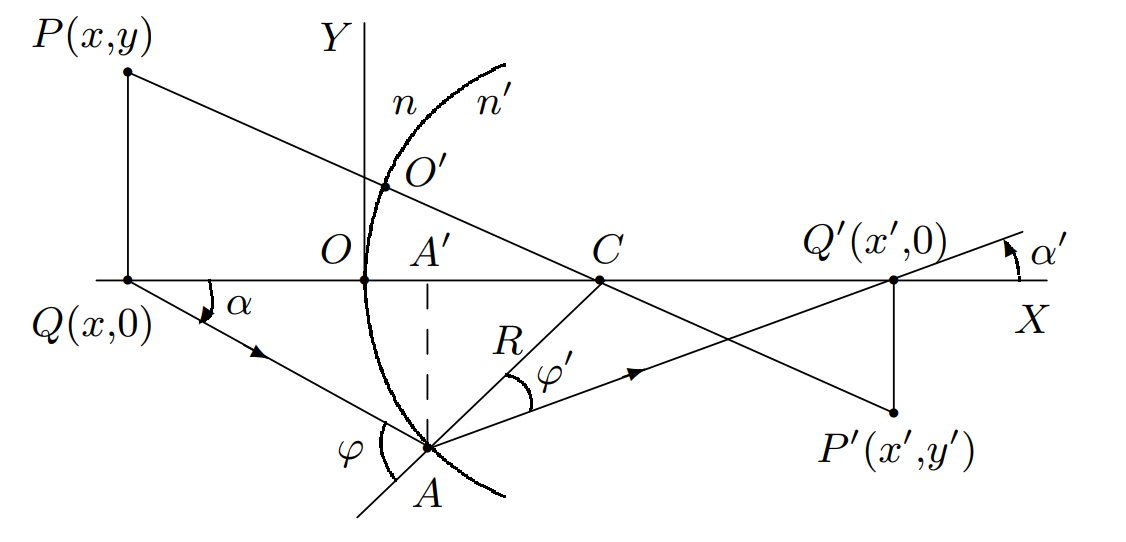
\includegraphics[width=0.8\linewidth]{Screenshot_1}
		\caption{Элементарная оптическая ячейка}
		\label{2}
	\end{figure}
	
	
	Используя закон преломления, получим для элементарной оптической ячейки, изображённой на \picref{2}, в параксиальном приближении:
	\begin{equation}\label{опт-ячейка}
		-\frac{n}{x}+\frac{n'}{x'} = \frac{n'-n}{R},
	\end{equation}
	\begin{equation}
		x \alpha = x' \alpha'.
	\end{equation}
	Для прямой $ P P' $, рассмотренной как оптическая ось, 
	\begin{equation}\label{PP}
		\frac{y'}{y} = \frac{x' - R}{x - R}.
	\end{equation}
	
	Проведя замену переменных, получим систему уравнений
	\begin{equation}\label{grid}
		\frac{x' - F'}{H' - F'}= \frac{H-F}{x- F} = \frac{y'}{y} = \frac{n \alpha}{n' \alpha'},
	\end{equation}
	\begin{equation}\label{grid1}
		(x-H)\alpha= (x' - H')\alpha'.
	\end{equation}
	Из этих уравнений получим
	\begin{equation}\label{Ф}
		\frac{n}{f} = -\frac{n'}{f'} \equiv \Phi,
	\end{equation}
	где
	\begin{equation}\label{focus-len}
		f\equiv H - F, \;\;\; f'\equiv H' - F'.
	\end{equation}
	$ f $ и $ f' $ -- главные фокусные расстояния системы.
	
	
	
	
	
	\subsection{Определение фокусного расстояния тонкой собирающей линзы и сложных оптических систем по методу Аббе}
	
	Схема, применяемая для определения фокусного расстояния $ F $ оптической системы по методу Аббе, изображена на \picref{1}.
	\begin{figure}[tbp]
		\centering
		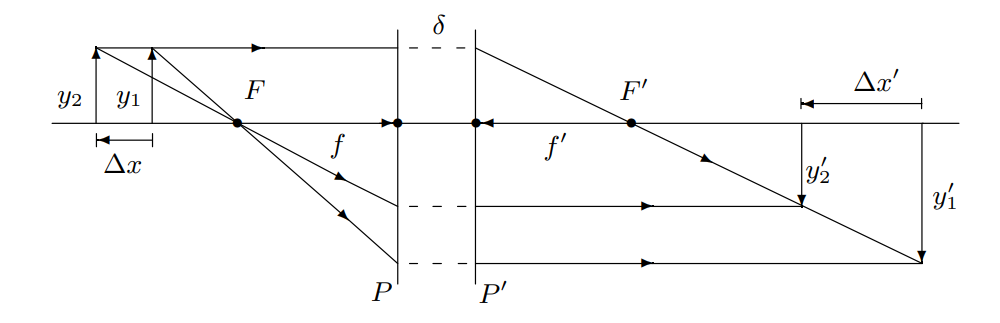
\includegraphics[width=0.8\linewidth]{Screenshot_3}
		\caption{Иллюстрация метода Аббе}
		\label{1}
	\end{figure}
	
	Из формул \eqref{Ф}, \eqref{grid}, \eqref{focus-len} получим:
	\begin{equation}\label{abbe}
		f = \frac{\Delta x}{\Delta (y/y')} = -\frac{\Delta x'}{\Delta (y'/y)}.
	\end{equation}
	
	\subsection{Определение фокусного расстояния собирающих линз и сложных оптических систем по методу Бесселя}
	
	\begin{figure}[tbp]
		\centering
		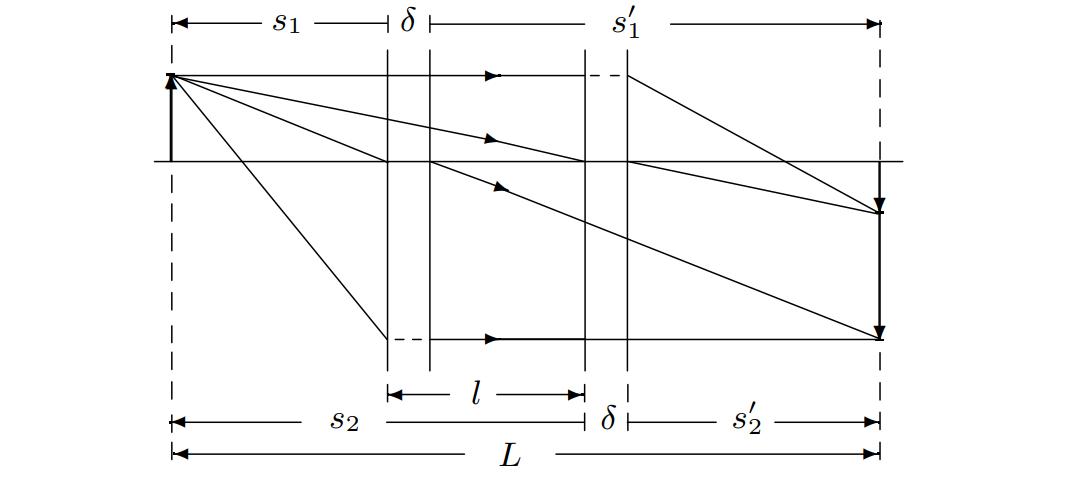
\includegraphics[width=0.8\linewidth]{Screenshot_2}
		\caption{Иллюстрация метода Бесселя}
		\label{3}
	\end{figure}
	Схема метода Бесселя для случая, когда $n = n'$ и $f' = -f$, представлена на \picref{3}. Тогда фокусное расстояние вычисляется по формуле:
	\begin{equation}\label{Bessel}
		f = \frac{(L - \delta)^2 - l^2}{4(L-\delta)}.
	\end{equation}
	
	В данной работе предпочтение отдаётся методу Аббе.
	
	\subsection{Определение фокусного расстояния тонкой собирающей линзы}
	
	\paragraph{Способ 1.} Воспользуемся формулой тонкой линзы:
	\begin{equation}\label{thin-lens}
		-\frac{1}{a}+\frac{1}{a'} = \frac{1}{f}.
	\end{equation}
	\paragraph{Способ 2.}
	Фокусное расстояние тонкой собирающей линзы можно определить с помощью зрительной трубы, настроенной на бесконечность, то есть на параллельный пучок лучей. Разместив между предметом и зрительной трубой положительную линзу и перемещая её вдоль оси системы, можно найти резкое изображение предмета в окуляре зрительной трубы. При этом расстояние от середины линзы до предмета равно фокусному расстоянию тонкой линзы.
	
	\subsection{Определение фокусного расстояния тонкой рассеивающей линзы}
	
	\paragraph{Способ 1.} Сначала с помощью собирающей линзы получают на экране действительное изображение предмета $ S $ (точка $ S_1 $ на \picref{4}). Затем на пути лучей, выходящих из собирающей линзы, располагают исследуемую рассеивающую линзу и, отодвигая экран, получают чёткое изображение предмета на экране, образованное двумя линзами. Точка $ S_1 $ пересечения сходящихся лучей играет по отношению к рассеивающей линзе роль мнимого источника. Изображение источника переместится теперь в точку $ S_2 $. 
	
	\begin{figure}[tbp]
		\centering
		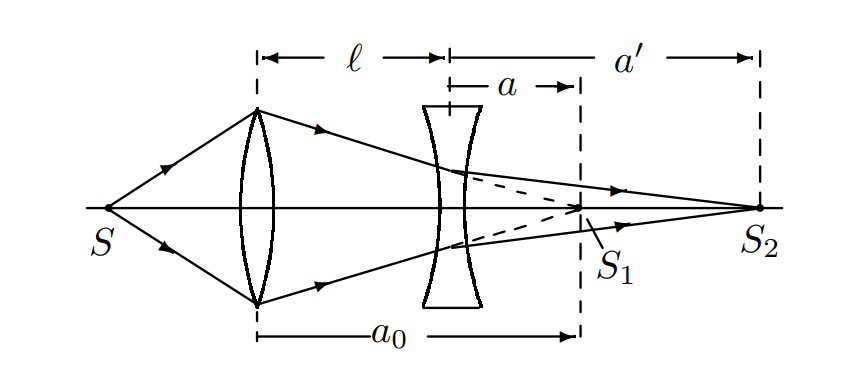
\includegraphics[width=0.8\linewidth]{Screenshot_5}
		\caption{Определение фокусного расстояния тонкой рассеивающей линзы}
		\label{4}
	\end{figure}
	
	
	Определив расстояния $ a = a_0 - l > 0$ и $ a'>0 $, рассчитывают фокусное расстояние рассеивающей линзы по формуле \eqref{thin-lens}.
	
	\paragraph{Способ 2}
	
	Если расстояние $ a $ на \picref{4} совпадает с модулем фокусного расстояния рассеивающей линзы, то изображение $S_2$ перемещается в бесконечность, то есть лучи выходят из линзы параллельным пучком. Параллельность пучка можно установить с помощью зрительной трубы, настроенной на бесконечность. Зная расстояние от первой линзы до точки $S_1$ и расстояние между линзами, нетрудно определить фокусное расстояние тонкой рассеивающей линзы. Для толстой отрицательной линзы этот метод позволяет определить только положение главного фокуса.
	
	
	\subsection{Определение положения главных и фокальных плоскостей сложной оптической системы}
	
	Для нахождения главных плоскостей системы недостаточно знать фокусное расстояние, нужно определить ещё положения главных фокусов. Это можно сделать при помощи зрительной трубы, настроенной на бесконечность. Отложив от главных фокусов отрезки, равные фокусному расстоянию, можно найти положения главных плоскостей системы. При этом необходимо учитывать возможность различного взаимного расположения кардинальных точек (плоскостей) сложной системы.
	\section{Ход работы}
	Перед началом измерений проведем калибровку оптической с помощью поперечных салазок на линзах, а также выровняем изображение на экране.
	\subsection{Измерение фокусного расстояния линзы 1 (собирающей)}
	\subsubsection{Метод Аббе}
	Произведем замеры передвигая источник на небольшое расстояние и фиксируя сдвиг изображения. Замерим расстояния согласно обозначениям на \picref{1}.
	\begin{table}[H]
		\centering
		\begin{tabular}{|l|l|l|l|l|l|l|l|l|l|l|}
			\hline
			  y, см   &  $y_1^\prime$, см   &    $y_2^\prime$, см   &  $x_2$, см  &  $x_1$, см   &   $\Delta x$, см                        &     $x_2^\prime$, см                      &       $x_1^\prime$, см                   &    $\Delta x^\prime$, см                       &         $f$, см & $f^\prime$, см                  \\ \hline
			2 & 3.2 & 5.1 & 27.6 & 25 & 2.6 & \multicolumn{1}{c|}{84.4} & \multicolumn{1}{c|}{74.6} & \multicolumn{1}{c|}{9.8} & \multicolumn{1}{c|}{11.2} & \multicolumn{1}{c|}{10.3} \\ \hline
		\end{tabular}
		\caption{Измерение фокусного расстояния линзы 1 по методу Аббе}
	\end{table}
	\subsubsection{Метод Бесселя}
	Проведем измерение по методу Бесселя с различными расстояниями от источника до оптической системы.
	\begin{table}[H]
		\centering
		\begin{tabular}{|l|l|l|l|l|}
			\hline
		$L$, см	&    $a_1$, см  &   $a_2$, см   &  $l$, см    &  $f$, см     \\ \hline
			57.5 & 17.2 & 43.8 & 26.6 & 11.30 \\ \hline
			62.5 & 16.6 & 49.2 & 32.6 & 11.37 \\ \hline
			67.5 & 16   & 54.5 & 38.5 & 11.39 \\ \hline
		\end{tabular}
		\caption{определение фокусного расстояние линзы 1 методом Бесселя}
	\end{table}
	Среднее значение фокуса: $\bar{f}$ = 11.35 см. При этом среднеквадратичное отклонение получилось равным: $\sigma_f$ = 0.67 мм. Это говорит о хорошей репрезентативности результатов полученных этим методом.
	\subsubsection{Формула тонкой линзы}
	Построили систему из экрана, источника и линзы, замерим расстояния и по формуле тонкой линзы: a = 13.6 см, b = 36.5 см, f = 9.91 см
	\subsection{Измерение фокусного расстояния рассеивающей линзы 4}
	Для измерения фокусного расстояния рассеивающей линзы воспользуемся вспомогающей собирающей линзой 1, фокусное расстояние которой мы замерили ранее.
	\begin{table}[H]
		\centering
		\begin{tabular}{|c|c|c|c|c|}
			\hline
		$a_0$, см	&  $l$, см    &   $a = a_0 - 1 $, см  & $a^\prime$, см   & $f$, см    \\ \hline
			35.4 & 28.9 & 6.5 & 13 & -13 \\ \hline
		\end{tabular}
		\caption{определение фокусного расстояния рассеивающей линзы 4}
	\end{table}
	\subsection{Измерение фокусов линзы при помощи зрительной трубы}
	По источнику света в конце длинного коридора проведем настройку зрительной трубы на бесконечность. Будем производить измерения фокусного расстояния с целью проверить можем ли мы считать наши линзы тонкими, путем замера фокусного расстояния линзы и последующего ее переворота.
	\paragraph{Линза 1 (собирающая)} 
	Первый замер: $f$ = 10.5 см, после переворота линзы $f$ = 10.4 см.
	\paragraph{Линза 2 (собирающая)} 
	Первый замер: $f$ = 13.9 см, после переворота линзы $f$ = 14.4 см.
	\paragraph{Линза 4 (рассеивающая)} 
	Первый замер: $a_0$ = 37.5 см, $l$ = 23.6 см, $f$ = -12.1 см, перевернем линзу, новые значения: $a_0$ = 35.7 см, $l$ = 23.9 см, $f$ = -11.8 см.\\
	
	По полученным значениям можем сказать, что данные нам линзы являются тонкими.
	Усредняя значения получим для фокусных расстояний измеренных с помощью оптической трубы: $f_1$ = 10.5 см, $f_2$ = 14.2 см, $f_4$ = -12 см.
	\subsection{Измерение характеристик сложной оптической системы}
	Измерим фокусное расстояние сложной системы при помощи источника и экрана и рассчитаем теоретически.
	\begin{table}[H]
		\centering
		\begin{tabular}{|l|l|l|l|l|l|l|l|l|l|l|l|}
			\hline
			$\Delta$, см&y, см   &  $y_1^\prime$, см   &    $y_2^\prime$, см   &  $x_2$, см  &  $x_1$, см   &   $\Delta x$, см                        &     $x_2^\prime$, см                      &       $x_1^\prime$, см                   &    $\Delta x^\prime$, см                       &         $f$, см & $f^\prime$, см                  \\ \hline
			5.4 & 2 & 6.7 & 1.8 & 16.5 & 10.3 & 6.2 & \multicolumn{1}{c|}{93.5} & \multicolumn{1}{c|}{75.9} & \multicolumn{1}{c|}{17.6} & \multicolumn{1}{c|}{7.63} & \multicolumn{1}{c|}{7.18} \\ \hline
		\end{tabular}
		\caption{Измерение фокусного расстояния сложной системы}
	\end{table}
	Итого по результатам замеров получили: $f$ = 7.41 $\pm$ 0.06 см.\\
	Из теоретических расчетов получаем: $f$ = 7.73 см.\\
	Видим что получили сходные значения, однако оценка погрешности измерения длины оказывается заниженной, что оказывает влияние на итоговую погрешность.
	\subsubsection{Определение главных и фокальных точек в пространстве изображений сложной оптической системы}
	Проведем замеры и получим значения теоретически полагаясь на: $l$ = 5.4 см, $f_1$ = 10.5 см, $f_2$ = 14.2 см, $\Delta$ = -19.3 см.
	\paragraph{Теория} $H_1$ = 2.94 см, $H_2$ = -3.97 см, $F_1$ = -4.79 см, $F_2$ = 3.75 см.
	\paragraph{Практика} $H_1$ = 3 см, $H_2$ = -4.1 см, $F_1$ = -4.5 см, $F_2$ = 3.1 см.\\
	Заметим что результаты эксперимента сходятся с теоретической оценкой.
	\section{Выводы}
	1) В ходе работы были изучены основные методы измерения фокусных расстояний центрованных оптических систем.\\
	2) Измерили фокусное расстояние тонкой собирающей линзы (1) тремя способами: метод Аббе - 10.3 см, метод Бесселя - 11.4 см, формула тонкой линзы - 9.9 см, зрительная труба настроенная на бесконечность - 10.5 см. Все полученные результаты отличаются не более чем на 20\%, что косвенно указывает на их справедливость. Наилучшую точность получили методом Бесселя, так как среднеквадратичное отклонение между разными замерами составило не более 0.67 мм.\\
	3) Для рассеивающей линзы (4): при помощи системы двух линз - (-13) см, с помощью зрительной трубы - (-12) см. Разница в результатах составляет 8\%, что может говорить о справедливости наших замеров.\\
	4) В пункте 3.4 получили характеристики сложной оптической системы, составленной из двух линз. В случае наших расчетов теория от практики отличается на 17\% в случае координат и на 4\% для расчета фокусного расстояния.\\
\end{document}